% =============================================================================
%  s04b-fukaya.tex —— 第 4 节后半部分（§4.5--§4.8）
%  《A Symplectic Prolegomenon》(Ivan Smith, arXiv:1401.0269v2) 中文译注版
%  对应源码 p0269/src/Prolegomenon_utf8.tex 第 1165--1368 行
%  说明：本文件不含 \section 与 keypoints（节首由 s04a-fukaya.tex 负责），
%        直接从 §4.5 起排。
% =============================================================================

\subsection{分类策略}

理解给定辛流形 $(X,\omega)$ 的 Fukaya 范畴的一种策略包含三个基本步骤：选定一族“钟爱的”拉格朗日子流形 $\{L_i\}$；计算有限维代数 $\oplus_{i,j} HF^*(L_i, L_j)$ 上的 $A_{\infty}$-结构；然后证明 $\{L_i\}$（分裂）生成 $\scrF(X)$。核心的一步往往迂回进行，以尽量减少对 Cauchy--Riemann 方程显式解的需要。

\subsubsection{Hochschild 上同调}

$A_{\infty}$-范畴的 \emph{Hochschild 上同调}由如下的 bar 复形 $CC^*(\scrA,\scrA)$ 定义。次数为 $r$ 的上链是一个序列 $(h^d)_{d\geq 0}$，其中每一项是一族线性映射
\[
h^d_{(X_1,\ldots,X_{d+1})}: \bigotimes_{i=d}^1 hom_{\scrA}(X_i,X_{i+1}) \rightarrow hom_{\scrA}(X_1,X_{d+1})[r-d]
\]
对每个 $(X_1,\ldots,X_{d+1})\in \Ob(\scrA)^{d+1}$ 给出。微分由对拼接求和定义：
% [Tutor Note: $\maltese_i=\sum_{j=1}^i|a_j|-i$ 是定义 $A_\infty$ 关系时引入的 Koszul 符号（见第 2 节）。
%   Hochschild 微分的两项分别对应“在外层插入 $\mu$”与“先在内层插入 $\mu$”，符号 $(r+1)\maltese_i$ 与 $\maltese_i+r+1$ 极易记反；
%   核对办法是取 $d=2$ 的小情形逐项验证 $\partial^2=0$，并留意 $r$ 作为 $h$ 次数的整体移位始终保留在指数中。]
\begin{equation} \label{Eqn:Hochschild}
\begin{aligned}
(\partial h)^d & (a_d,\ldots, a_1) = \\
& \sum_{i+j<d+1} (-1)^{(r+1)\maltese_i} \mu_{\scrA}^{d+1-j}(a_d,\ldots,a_{i+j+1},h^j(a_{i+j},\ldots,a_{i+1}),a_{i},\ldots,a_1) \\
+ &  \sum_{i+j\leq d+1} (-1)^{\maltese_{i} +r +1}  h^{d+1-j} (a_d,\ldots,a_{i+j+1},\mu_{\scrA}^j(a_{i+j},\ldots,a_{i+1}),a_{i},\ldots,a_1).
\end{aligned}
\end{equation}
更简洁地说，事实上 $HH^*(\scrA,\scrA) = H(hom_{fun(\scrA,\scrA)}(\id,\id))$。域上 $A_{\infty}$-范畴的 Hochschild 上同调在取扭曲复形与幂等完备化之下均不变 \cite[Section 1c]{Seidel:Flux}。
% [Tutor Note: 把 $HH^*(\scrA,\scrA)$ 写成恒等函子的自同态复形的上同调，采用的是函子范畴中以 $\mu^1$ 为微分的标准约定；
%   它与 bar 复形的上同调同构，但具体上链的符号与次序约定可能相差一个符号，跨文献比较 $HH^*$ 的元素时必须先对齐约定。]

设 $A$ 是域 $\bK$ 上的 $\bZ_2$-分次代数，$\bK$ 的特征不等于 2。我们关心 $A$ 上微分平凡的那些 $\bZ_2$-分次 $A_{\infty}$-结构。这样的结构由一族映射
\[
\{ \alpha^i: A^{\otimes i} \rightarrow A \}_{i\geq 2}
\]
组成，其中 $\alpha^i$ 的奇偶性为 $i$。我们引入模 2 分次的 Hochschild 上链复形
\[
CC^{\bullet+1}(A,A) \ = \ \prod_{i \geq 2} Hom^{(\bullet+i)}(A^{\otimes i},A)
\]
其中 $Hom^{(\bullet +i)}$ 表示我们考虑奇偶性为 $\bullet+i$ 的同态。它带有通常的微分 $d_{CC^{\bullet}}$ 与 Gerstenhaber 括号 $[\cdot, \cdot]$。$A$ 上延拓其给定乘法的 $A_{\infty}$-结构 $(\alpha^i)$ 对应于满足 Maurer--Cartan 方程
\begin{equation} \label{Eqn:Maurer-Cartan}
d_{CC^{\bullet}} (\alpha) + \frac{1}{2} [\alpha, \alpha] = 0\qquad \textrm{with} \quad \alpha^1 = \alpha^2 = 0.
\end{equation}
的 $CC^{1}(A,A)$ 中元素 $\alpha$。
% [Tutor Note: 条件 $\alpha^1=\alpha^2=0$ 表示新的 $A_\infty$-结构保留原有乘法与零微分，只从 $\alpha^3$ 起才可能有非零项；
%   “规范变换”只在适当收敛条件下有效，实践中 $\bK$ 取 Novikov 域或 $\alpha$ 幂零时即可。]

$CC^0(A,A)$ 中的元素 $(g^i)_{i\geq 1}$（由奇偶性为 $i-1$ 的映射 $A^{\otimes i} \rightarrow A$ 组成）通过规范变换作用在 Maurer--Cartan 解集 $(\alpha^i)_{i\geq 2}$ 上，至少当适当的收敛性条件成立时如此。因此，给定代数 $A$ 上的 $A_{\infty}$-结构之集与 $A$ 的 Hochschild 上链复形紧密相联。为把这两种讨论联系起来：若 $\scrA$ 表示由 Maurer--Cartan 元素 $\alpha \in CC^1(A,A)$ 定义的 $A_{\infty}$-代数，且 $H(\scrA) = A$，则 $HH^*(\scrA,\scrA)$ 就是复形 $CC^{\bullet}(A,A)$ 关于扭微分 $d_{CC^{\bullet}} + [\cdot, \alpha]$ 的上同调。

由 \eqref{Eqn:ClosedOpen} 给出的闭-开弦映射 $\mathcal{CO}^0: QH^*(X) \rightarrow HF^*(L,L)$ 可以延拓为映射：只需考虑带有内部输入、若干边界输入以及单个边界输出的圆盘，
\begin{equation} \label{Eqn:COHH}
\mathcal{CO}: QH^*(X) \longrightarrow HH^*(\scrF(X), \scrF(X))
\end{equation}
我们仍称之为闭-开弦映射；将它与此前投影到 Hochschild 复形长度零部分的截断映射复合，就还原出先前引入的映射 \eqref{Eqn:ClosedOpen}。

\begin{Remark}\label{Rem:StarC1}
在 \ref{Subsec:ModuleStructures} 节中我们曾指出，Auroux、Kontsevich 与 Seidel 证明了：对单调辛流形，Fukaya 范畴 $\scrF(X)$ 可能的直和项被 $\ast c_1(X)$ 的特征值所指标。形式地，他们的论证始于如下观察：复合
\[
\mathcal{CO}^0: \ QH^*(X) \longrightarrow HH^*(\scrF(X), \scrF(X)) \longrightarrow HF^*(L,L)
\]
即 \eqref{Eqn:COHH} 与到 Hochschild 复形长度零部分的截断之复合，满足
\begin{equation} \label{Eqn:2c1degrees}
\mathcal{CO}^0(2c_1(X)) = 2 \frak{m}_0(L) \in HF^*(L,L).
\end{equation}
回忆在 $H^2(X,L) \rightarrow H^2(X)$ 下 $\mu_L \mapsto 2c_1(X)$，并取 Maslov 圈 $\mu_L \in H^2(X,L) = H^2_{ct}(X\backslash L)  \cong H_{2n-2}(X\backslash L)$ 的一个与 $L$ 不相交的代表 $D$，以消去常值圆盘的贡献，则 \eqref{Eqn:2c1degrees} 的两边本质上计数同一对象：一个边界落在 $L$ 上、内部标记点被约束在 $D$ 上的 Maslov 指标 2 圆盘。由指标原因，$\frak{m}_0(L) \in HF^*(L,L)$ 是单位元 $e_L$ 的倍数（同义反复地，若 $L$ 不界定任何 Maslov 指标 2 圆盘，则为零倍）。若 $\frak{m}_0(L) = \lambda e_L$，则
\[
QH^*(X) \rightarrow HF^*(L,L) \quad \mathrm{takes} \ 2(c_1-\lambda 1) \mapsto 0
\]
从而在特征 $\neq 2$ 时，$c_1-\lambda 1$ 不可逆。
\end{Remark}

\subsubsection{有限确定性\label{Subsec:FiniteDeterminacy}}

正如 Floer 上同调上的乘法在链层面有底层的 $A_{\infty}$-结构，Hochschild 上同调上的 Lie 括号在链层面有底层的 $L_{\infty}$-结构。Kontsevich 的形式性定理 \cite{Kontsevich:DefQuant} 断言：若 $A$ 是光滑交换代数，则在适当的滤过幂零条件下存在 $L_{\infty}$-代数的拟同构 $CC^*(A,A) \rightarrow HH^*(A,A)$，它在 Maurer--Cartan 解集上诱导双射。这使人能把 $A$ 上 $A_{\infty}$-结构的存在性与分类结果，转化为关于 Hochschild 上同调以及规范变换在其上作用的问题。

取 $A = \Lambda(V)$ 为有限维外代数可很好地说明这一结论。Hochschild--Kostant--Rosenberg 定理把 Hochschild 上同调等同于 $V$ 上多重向量场的 Lie 代数，即
\[
Sym^{\bullet}(V^{\vee}) \otimes \Lambda(V) \ = \ \bC[\![V]\!] \otimes \Lambda(V).
\]
其 Lie 代数结构来自 Schouten 括号
\begin{equation}
\begin{aligned} {}
& [f \,\xi_{i_1} \wedge \cdots \wedge \xi_{i_k}, g \,\xi_{j_1} \wedge \cdots \xi_{j_l}] = \\
& \textstyle \qquad \sum_q (-1)^{k-q-1} f \, (\partial_{i_q}g) \,
\xi_{i_1}  \wedge \cdots \wedge \widehat{\xi_{i_q}} \wedge \cdots
\wedge \xi_{i_k} \wedge \xi_{j_1} \wedge \cdots \wedge \xi_{j_l} + \\ & \textstyle \qquad
 \sum_q (-1)^{l-q+ (k-1)(l-1)} g \,(\partial_{j_q}f)\, \xi_{j_1} \wedge \cdots \wedge \widehat{\xi_{j_q}} \wedge \cdots \wedge \xi_{j_l} \wedge \xi_{i_1} \wedge
 \cdots \wedge \xi_{i_k}.
\end{aligned}
\end{equation}
由于 Schouten 括号在函数上为零，Kontsevich 定理蕴含：任何形式函数 $W\in\bC[\![V]\!]$ 定义一个 Maurer--Cartan 解，从而定义 $\Lambda(V)$ 上的一个 $A_{\infty}$-结构；并且相差一个形式微分同胚的拉回的两个函数，定义拟同构的 $A_{\infty}$-结构。

现设 $W$ 在 $0\in V$ 处有孤立临界点。于是奇点的经典有限确定性理论蕴含：$W$ 在形式坐标变换下等价于一个多项式。在这个意义上，由 $W$ 定义的 $A_{\infty}$-结构被有限量的数据完全决定（在拟同构意义下），从原则上说是可计算的，尽管 \emph{a priori} 它可能允许无穷多个非零乘积。有关一个概览性的例子见 \ref{Subsec:genus2} 节。
% [Tutor Note: 有限确定性保证 $W$ 经形式坐标变换可化为多项式，其次数 $d$ 给出上界：只有 $k\le d$ 时 $\mu^k$ 才可能非零，
%   因此尽管 $\mu$ 的指标集为无限，实际非零的乘积只有有限多个。“最高次非零 $\mu^k$”指 $k$ 最大的那个非零乘积，
%   它对应多项式最高次项经缩并所得的最后一层运算，其后再无更高阶乘积；不同多项式代表给出的结构在拟同构意义下相同。]

\subsection{生成\label{Sec:Generation}}

拥有一个判别有限族拉格朗日子流形生成 Fukaya 范畴的判据是重要的。具体地，给定 $L_1,\ldots,L_k \subset X$，有 $A_{\infty}$-代数
$\scrA \ = \ \oplus_{i,j} HF^*(L_i,L_j)$。
称 $L_i$ 分裂生成 $\scrF(X)$，若 $\scrF(X)$ 的每个对象都拟同构于 $\{L_i\}$ 上某个扭曲复形的一个直和项；这蕴含函子
\[
\scrF(X) \longrightarrow  \mathrm{mod}_{\!A_{\infty}}(\scrA), \qquad K \mapsto \oplus_i \, HF^*(K,L_i)
\]
是全忠实嵌入。我们将提到两个充分判据；后者更强，但前者在某些有趣的情形中适用。

\subsubsection{正关系}

先设 $\{L_1,\ldots, L_k\} \subset X$ 都是拉格朗日球面，并且满足一个 \emph{正关系}，即正 Dehn 扭转 $\tau_{L_i}$ 中的某个字 $w \in \langle \tau_{L_1}, \ldots, \tau_{L_k}\rangle$ 与恒等映射 Hamilton 同痕。字 $w$ 连同该同痕给出一个辛 Lefschetz 纤维化 $\scrX \rightarrow \bP^1$，其一般纤维辛同胚于 $X$，在 $\bC \subset \bP^1$ 上的单值性由 $w$ 给出，并经由给定的 Hamilton 同痕补全为 $\infty \in \bP^1$ 上的纤维化。坚持同痕是 Hamilton 的（而不只是辛的）之要点在于：$\scrX$ 的全空间此时带有延拓了来自 $X$ 的逐纤维结构的辛结构。特别地，$\scrX$ 中有良好的全纯曲线理论。

在陈述下述命题时，我们假设 $X$ 是单调的并在 $\bC$ 上工作，于是如注 \ref{Rem:StarC1} 那样，$\scrF(X) = \oplus_{\lambda} \scrF(X;\lambda)$，其中 $\lambda \in \mathrm{Spec}(\ast c_1(X))$。
% [Tutor Note: 正关系 $w\in\langle\tau_{L_i}\rangle$ 与恒等 Hamilton 同痕给出 $\scrX\to\bP^1$：$\bC$ 上的单值性为 $w$，$\infty$ 处由同痕补全。
%   圈类 $\mathcal{C}(w)\in QH^*(X)$ 的定义是“把 $\scrX\to\bP^1$ 的全纯截面在基点处取值”：截面族在纤维 $X$ 中扫出该圈。
%   它可视作 $w$ 所定义自等价在闭弦层面（量子上同调）的图形；“$\mathcal{C}(w)$ 幂零”刻画该自等价在相应直和项上的幂零性。]

\begin{Proposition} \label{Prop:SpheresGenerate}
令 $\mathcal{C}(w) \in QH^*(X)$ 表示把 $\scrX\rightarrow \bP^1$ 的全纯截面在某基点处取值所得的圈。设所有 $L_i$ 都属于 $\scrF(X; \lambda)$，且 $QH^*(X;\lambda) $ 上以 $\mathcal{C}(w)$ 作的量子上杯积是幂零的。则 $\{L_i\}$ 分裂生成 $\scrF(X;\lambda)$。特别地，若 $\lambda =0$ 且 $\mathcal{C}(w)$ 是 $c_1(X)$ 的倍数，则 $L_j$ 分裂生成 $\scrF(X;0)$。
\end{Proposition}

\begin{proof}
由代数 Dehn 扭转与几何 Dehn 扭转之间的对应（命题 \ref{Prop:twists}），存在正合三角
\[
\cdots \rightarrow  HF(L,K)\otimes L \rightarrow K \rightarrow \tau_L(K) \stackrel{[1]}{\longrightarrow} \cdots
\]
其中 $K \subset X$ 是范畴的 $\lambda$-直和项中的任意拉格朗日子流形。如 \eqref{Eqn:RollTriangle} 那样把 $w$ 中出现的 $\tau_{L_j}$ 对应的三角拼接起来，定义一个自然映射
\begin{equation}\label{eqn:concatenate}
K \rightarrow \prod_{i_j} \tau_{L_{i_j}} K \cong K
\end{equation}
它由 $HF^*(K,K)$ 的一个元素给出。从 Floer 上同调中长正合列的最初构造 \cite{Seidel:LES} 以及 \ref{Subsec:ExactTriDon} 节可知，自然映射 $K \rightarrow \tau_L(K)$ 来自计数一个环带上带单个临界点的 Lefschetz 纤维化的截面。粘合定理 \cite[Proposition 2.22]{Seidel:LES} 蕴含：这类映射的拼接计数了把若干这样的环带缝在一起所得的 Lefschetz 纤维化的全纯截面。在自然限制映射 $r: H^{*}(M) \rightarrow HF^{*}(K,K)$ 下，方程 \ref{eqn:concatenate} 由圈类 $r(\mathcal{C}(w)) \in HF^{*}(K,K)$ 的像作乘法给出。若 $\mathcal{C}(w)$ 消失，则迭代正合三角中的一个映射消失，于是 $K$ 是 $\{L_i\}$ 中若干对象的迭代锥的一个直和项。若 $\ast \mathcal{C}(w)$ 幂零，则把 $w$ 换成 $w^N$（$N \gg 0$）后可重复同一论证。
\end{proof}
% [Tutor Note: 证明中写作 $r: H^{*}(M)\to HF^{*}(K,K)$，但全文流形记为 $X$，$M$ 应为早期记号残留；
%   论证只用到限制映射的存在性与幺性，按 $r: H^{*}(X)\to HF^{*}(K,K)$ 理解即可。]

\subsubsection{Abouzaid 判据}

命题 \ref{Prop:SpheresGenerate} 的明显缺陷在于 $L_i$ 必须是球面。Abouzaid \cite{Abouzaid:generation} 在恰当情形给出了更好的判据，一般而言则由 Abouzaid--Fukaya--Oh--Ohta--Ono（准备中）给出；对单调流形，后者的解释见 \cite{RitterSmith, Sheridan3}。

\begin{Theorem}[Abouzaid-Fukaya-Oh-Ohta-Ono] \label{Thm:AFOOOgenerate}\label{Thm:Generation}
若映射 $\mathcal{CO}: QH^*(X) \rightarrow HH^*(\scrA,\scrA)$ 是同构，则 $L_i$ 分裂生成 $\scrF(X)$。
\end{Theorem}
% [Tutor Note: 判据的实质是“闭-开弦映射命中单位 $\Rightarrow$ 分裂生成”。$\mathcal{CO}$ 为同构时 $QH^*(X)$ 的单位映为 $HH^*$ 的单位，
%   而 $HH^*$ 的单位含于 $\{L_i\}$ 所生成的对象之中，故每个对象都是 $\{L_i\}$ 的扭曲复形的直和项。
%   注意 $\mathcal{CO}$（到 $HH^*(\scrA,\scrA)$）与 $\mathcal{CO}^0$（到 $HF^*(L,L)$）是不同层级的映射，切勿混用。]

考察定理 \ref{Thm:Generation} 所论情形的一个玩具模型是有启发性的：它只在 Hochschild 上同调的长度零部分层面运作，此时 \eqref{Eqn:COHH} 的闭-开弦映射约化为先前考虑过的较简单的 \eqref{Eqn:ClosedOpen}。设存在拉格朗日子流形 $L\in \scrF(X;\lambda)$，使得
\[
\mathcal{CO}^0: QH^*(X;\lambda) \rightarrow HF^*(L,L)
\]
是同构。我们将证明此时 $L$ 分裂生成 $\scrF(X;\lambda)$。事实上，对任意 $K\in \scrF(X;\lambda)$，只需证明映射
\begin{equation} \label{Eqn:HitUnit}
HF^*(L,K) \otimes HF^*(K,L) \longrightarrow HF^*(K,K)
\end{equation}
命中单位元 $1_K$。为验证这一点，在 \eqref{Eqn:HitUnit} 中写 $1_K = \sum_{j=1}^N p_j \cdot q_j$。存在映射
\[
\alpha = \sum_{j=1}^N \mu^2(p_j, \cdot) \quad \mathrm{and} \quad \beta = (\mu^2(q_1,\cdot),\ldots, \mu^2(q_N,\cdot))
\]
它们构成图表
\[
\xymatrix{
\bigoplus_{j=1}^N \, HF^*(L,L)\ar@<+2pt>@{->}^-{\alpha}[rr] \ar@<-2pt>@{<-}_-{\beta}[rr] && HF^*(L,K)
& \alpha \circ \beta  =1_K} 
\]
这表明 $\beta \circ \alpha$ 是幂等的，其像同构于 $HF^*(L,K) \subset \oplus_j HF^*(L,L)$ 的一个拷贝。由此，$K \in \Tw^{\pi}\langle L\rangle $ 是 $L$ 的若干拷贝的直和项（拟同构于幂等元 $\beta\circ\alpha$ 的像，而该像在取分裂闭包时被形式地作为一个对象引入）。
% [Tutor Note: 这里把“$L$ 分裂生成”化归为“乘法 (4.x) 的像含有 $1_K$”：一旦 $1_K\in \mathrm{im}(\mu^2)$，$K$ 就是 $L$ 的扭曲复形的直和项。
%   构造幂等元 $\beta\circ\alpha$ 时 $\alpha,\beta$ 的次序与转置极易颠倒：$\alpha$ 以 $p_j$ 为第一个变量，$\beta$ 以 $q_j$ 为第一个变量，
%   二者配对给出 $1_K$，反过来得到的 $\beta\circ\alpha$ 只是 $HF^*(L,K)$ 上的投影。]

\begin{figure}[ht]
  \centering
  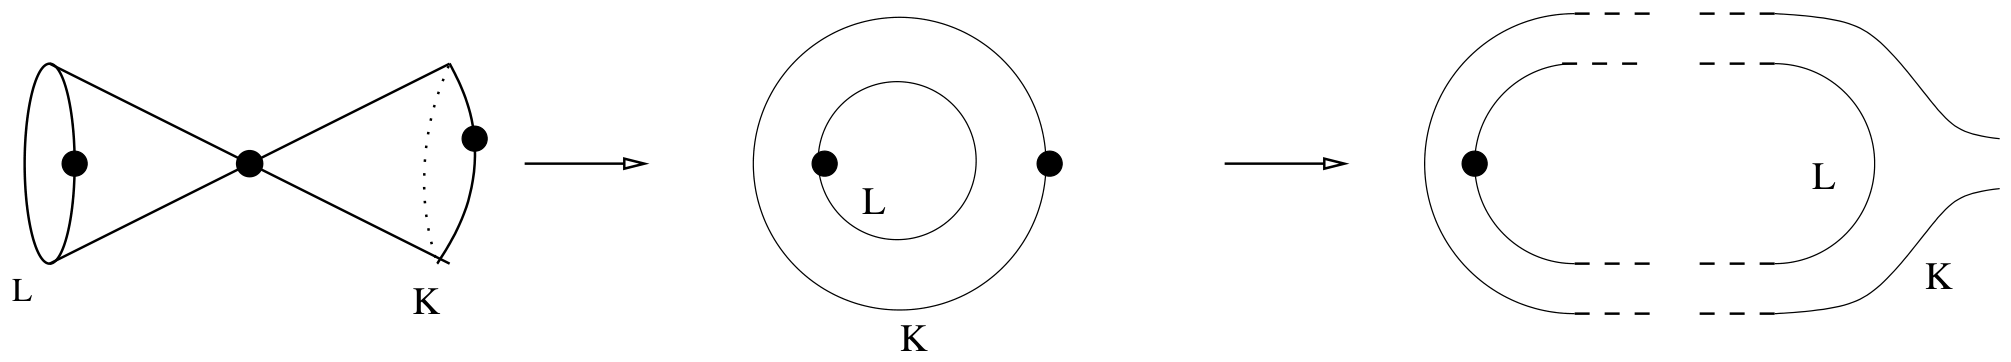
\includegraphics[width=0.85\textwidth]{fig11-cardy2.png}
  \caption{Cardy 关系的一个变体（原文 Figure~10，第 33 页）。\label{Fig:Cardy2}}
\end{figure}

为看出 \eqref{Eqn:HitUnit} 命中单位元，我们研究一参数族的环带，见图 \ref{Fig:Cardy2}（这类论证被称为 Cardy 关系，在此语境下可追溯到 \cite{BiranCornea}）。在该图左侧，我们在 $L$ 与 $K$ 的边界分支上固定标记点。把那个结点环带视为 $X\times X$ 中带原点处关联条件的圆盘，该图表示对角线的像
\begin{equation} \label{Eqn:Nodal}
\Delta \subset QH^*(X) \otimes QH^*(X) \longrightarrow HF^*(L,L) \otimes HF^*(K,K).
\end{equation}
若 tr$: HF^*(L,L) \cong QH^*(X;\lambda) \rightarrow \bC$ 是与基本类配对所给的 $QH^*(X)$ 上通常迹的限制，则我们因此得到一个类 $(\tr \otimes \id)(\Delta) \in HF^*(K,K)$。另一方面，图 \ref{Fig:Cardy2} 中间的环带（带有两个边界标记点）可沿一维退化的另一端分解为一条带一个边界标记点的条带与一个三穿孔圆盘。在此情形下，用 $HF^*(L,L)$ 上的迹封住该边界标记点，相当于考虑复合
\begin{equation} \label{Eqn:Smoothed}
\bK \rightarrow HF^*(L,K) \otimes HF^*(L,L) \otimes HF^*(K,L) \stackrel{\mathrm{tr}}{\longrightarrow} HF^*(L,K) \otimes HF^*(K,L) \stackrel{\mu^2}{\longrightarrow}HF^*(K,K). 
\end{equation}
通过这一参数族环带可以看出，$(\tr\otimes \id)(\Delta)$ 落在 \eqref{Eqn:Smoothed} 的像中，从而落在乘法 \eqref{Eqn:HitUnit} 的像中。由于对角线由 $[X]\otimes \id + $（其他项）给出，且 $QH^*(X) \rightarrow HF^*(K,K)$ 是幺的并透过 $QH^*(X;\lambda)$ 分解，比较 \eqref{Eqn:Nodal} 与 \eqref{Eqn:Smoothed} 即知 \eqref{Eqn:HitUnit} 的像包含单位元，正如所需。
% [Tutor Note: 对角类 $\Delta$ 的 Künneth 分解为 $[X]\otimes\id+$（其他项）：取 $\tr\otimes\id$（$\tr$ 为与基本类配对所得的迹）后，
%   $[X]\otimes\id$ 一项给出 $1_K$，而“其他项”经比较 (4.x) 与 (4.x) 可知已包含在乘法像中，这正是 (4.x) 命中单位的机制。
%   易错处：$QH^*$ 的分次移位与迹只取最高次分量的约定——按次数配对，低次项不进入单位。]

\subsection{应用 III}

我们继续贯穿全篇的主题：在一些典型情形中展示该代数机器；分别见 \cite{FSS,Nadler} 与 \cite{AbouzaidSmith:plumbing}。

\subsubsection{邻近拉格朗日\label{Sec:NearbyLag}}

余切丛的每个恰当拉格朗日子流形在 Fukaya 范畴中都同构于零截面，这是一个非平凡的定理，因此紧 Fukaya 范畴只含一个对象。该结果的证明经由对一个更有趣的范畴的描述，该范畴纳入非紧的拉格朗日子流形，即余切纤维。要点在于这些纤维生成 Fukaya 范畴（的适当版本）；这一事实已在 \eqref{Eqn:FibresShouldGenerate} 中初现端倪。

在技术层面有若干不同的途径，但任何一种都导致下述结果。设 $L\subset T^*Q$ 是 Maslov 类为零的恰当拉格朗日。Floer 上同调群 $HF^*(T^*_xQ,L)$ 构成 $Q$ 上一个 $\Z$-分次向量空间的平坦丛，记为 $E_L$。对 $L\subset T^*Q$ 可联系一个底层的链层面对象，即 $Q$ 上一个 $\bZ$-分次的 $dg$-层 $\scrE_L$，其纤维为 $CF^*(L, T_x^*Q)$；并论证这一对应把 Fukaya 范畴 $\scrF(T^*Q)$ 全忠实嵌入 $Q$ 上分次 $dg$-层构成的范畴。计算层 Ext 的通常局部-整体谱序列为
\[
E_1 = H^*(Q; \mathcal{E}xt(\scrE_L,\scrE_L)) \ \Longrightarrow \ \mathrm{Ext}^*(H(\scrE_L), H(\scrE_L))
\]
由 $\scrF(T^*Q)$ 嵌入的全忠实性，目标群可等同于 Floer 上同调 $HF^*(L,L)$。谱序列的 $E_2$-页于是给出
\begin{equation} \label{eq:ss}
E_2^{rs} = H^r(Q;\End^s(E_L)) \Rightarrow H^*(L;\bK)
\end{equation}
其中 $\End^*(E_L)$ 是分次自同态丛。由于 $\pi_1(Q)=0$，$E_L$ 是平凡丛，故 $E_2$ 页是一个“盒子” $H^*(Q) \otimes \End(HF^*(T^*_x,L))$。$E_2$ 层的微分从 $(r,s)$ 指向 $(r+2,s-1)$，更高页类似。于是盒子的左下角与右上角必定存活到 $E_\infty$。由于 $E_{\infty}$ 集中在次数 $0\leq \ast \leq n=\mathrm{dim}(Q)$，推出 $HF^*(T^*_x,L) \iso \bK$ 必须是一维的，且投影 $L \rightarrow Q$ 的度为 $1$。据此，谱序列退化，得 $H^*(L;\bK) \iso H^*(Q;\bK)$。还有另一个谱序列
\begin{equation} \label{eq:ss2}
E_1 = H^*(Q; \mathcal{E}xt(\scrE_Q,\scrE_L)) \ \Longrightarrow \ HF^*(Q,L).
\end{equation}
% [Tutor Note: 谱序列论证的关键是“盒子”形状：$E_2^{rs}=H^r(Q;\End^s(E_L))$ 的非零区域是 $0\le r\le n$ 且 $s$ 有界的矩形，
%   而收敛目标 $H^*(L;\bK)$ 只在 $0\le *\le n$ 非零，故矩形左下角与右上角必然存活到 $E_\infty$，迫使 $HF^*(T_x^*Q,L)$ 为一维。
%   其中用到 $\pi_1(Q)=0$ 使 $E_L$ 平凡；否则要把局部系数系统一并纳入，单值性会改变 $E_2$ 页。]

类似的分析表明边缘同态在最高次 $n$ 上是同构；该边缘同态可借助 Floer 乘积来解释，由此得出
\[
HF^n(T_x^*Q, L) \otimes HF^0(Q, T_x^*Q) \longrightarrow HF^n(Q,L) 
\] 
是同构，对任意 $x\in Q$ 成立。于是存在元素 $\alpha \in HF^0(Q,L)$，使得
\[
\mu^2(\alpha,\cdot): HF^*(T_x^*,Q) \rightarrow HF^*(T_x^*,L)
\]
是同构；但由于纤维生成该范畴，这恰好说明 $\alpha$ 在 $\scrF(T^*Q)$ 中定义了 $Q$ 与 $L$ 之间的同构。
% [Tutor Note: 原文此处写 $HF^*(T_x^*,Q)$ 与 $HF^*(T_x^*,L)$，按上下文应为 $HF^*(T_x^*Q,Q)$ 与 $HF^*(T_x^*Q,L)$（$x\in Q$ 为基点）。
%   此处照抄原文以求保真，请勿径改。]

\subsubsection{映射类群\label{Sec:MCGIII}}

定理 \ref{Prop:twists} 的一部分是如下陈述：对任意对象 $L \in \scrF(X)$ 都存在的代数扭转函子 $T_L$，当 $L$ 是球面时可逆。该论证可纯粹代数地给出，并且当 $L=\Sigma$ 是任意整系数同调球面时同样适用。令 $M_{\Sigma} = T^*\Sigma\#T^*S^n$ 为把给定的余切丛作管道连接（plumbing）所得的流形，即把一个 $T^*\Sigma$ 的纤维封顶成一个闭拉格朗日球面（该手术可在 Stein 范畴中实施）。$\bZ_2$-分次的恰当 Fukaya 范畴 $\scrF(M_{\Sigma})$ 容许自函子 $T_{\Sigma}$，由于 $\Sigma$ 是同调球面，它是等价。容易看出该等价是无穷阶的。设 $\pi_1(\Sigma)$ 有限但非平凡。我们断言 $T_{\Sigma}$ \emph{不是}由任何紧支辛同胚诱导的，即 \emph{不存在几何 Dehn 扭转}。（我们引入 $M_\Sigma$ 是为了给出一个完全用闭拉格朗日、而不用非紧余切纤维的论证。）

令 $\iota: \tilde{\Sigma} \rightarrow \Sigma$ 表示万有覆叠，$\pi: \tilde{M}_{\Sigma} \rightarrow M_{\Sigma}$ 为诱导的覆叠。固定一个特征整除 $\iota$ 的指数的系数域 $\bK$。反设代数扭转 $T_{\Sigma}$ 由某个紧支辛同胚 $\tau$ 诱导。考察 $\tau \circ \tau$ 或其逆，并回忆方程 \ref{Eqn:Twist} 中扭转函子的定义，我们推断存在一个恰当拉格朗日子流形 $L \subset M_{\Sigma}$，它表示扭曲复形
\begin{equation} \label{Eqn:ImpossibleComplex}
\Sigma \leftarrow \Sigma \leftarrow S^n
\end{equation}
其中最左的箭头由乘以基本类 $[\Sigma]$ 给出，$S^n$ 是另一个核心分支。现在回忆例 \ref{Ex:CoveringSpace}。\eqref{Eqn:ImpossibleComplex} 在 $\scrF(\tilde{M}_{\Sigma})$ 中的原像由 $\tilde{\Sigma} \leftarrow \tilde{\Sigma} \leftarrow \pi^{-1}(S^n)$ 表示，其中\emph{左微分消失}：它由 $\Sigma$ 的基本类拉回得到，故按我们对 $\bK$ 的特征的选取，它在系数域 $\bK$ 中为零。

作为连通拉格朗日子流形 $L$ 在一个覆叠下的原像，$\pi^{-1}(L)$ 的所有分支都微分同胚，并且由覆叠变换相联系，从而是 $\scrF(\tilde{M}_{\Sigma})$ 的自等价。复形 $\Sigma \leftarrow S^n$ 是 $\Sigma$ 在 $S^n$ 中 Dehn 扭转下的像。因此，$\tilde{\Sigma}$ 与 $\tilde{\Sigma} \leftarrow \pi^{-1}(S^n)$ 都由连通拉格朗日表示，从而都是不可分解对象（我们在 $\bZ$-分次情形，且对连通拉格朗日 $HF^0$ 的秩为 $1$）。同样由例 \ref{Ex:CoveringSpace}，它们不在覆叠变换的同一轨道中：取与 $  \pi^{-1}(S^n)$ 的某个分支处的余切纤维作 Floer 上同调，Floer 群在一种情形秩为 $0$，在另一种情形秩为 $1$。上一段表明，在相差平移的意义下，
\begin{equation} \label{Eqn:SplitPreimage}
\pi^{-1}(L) \cong \tilde{\Sigma} \oplus \left( \tilde{\Sigma} \leftarrow \pi^{-1}(S^n) \right)
\end{equation}
在范畴 $\scrF(\tilde{M}_{\Sigma})$ 中成立。我们现已证明 \eqref{Eqn:SplitPreimage} 的右端不同构于单个覆叠群轨道内的不可分解对象之直和，这是矛盾。
% [Tutor Note: 论证骨架：若 $T_\Sigma$ 有几何实现，则 (4.x) 的扭曲复形由某个恰当拉格朗日 $L$ 表示；
%   覆叠后最左微分由 $[\Sigma]$ 拉回、按特征选取在 $\bK$ 中为零，于是 $\pi^{-1}(L)$ 分裂成两个不可分解对象之直和，而二者分属不同覆叠轨道，矛盾。
%   易错点：$\tau$ 与 $\tau^{-1}$ 对应的扭曲复形相差一次平移，会改变 $[\Sigma]$ 前的符号；选取 $\tau\circ\tau$ 正是为了消除这一歧义。]

\begin{Notes} 关于 $A_{\infty}$-代数与 Fukaya 范畴的背景，见 \cite{FCPLT, FO3}。关于 Hochschild 上同调与形变理论的论证，见 \cite{Seidel:HMSquartic, Seidel:HMSgenus2}。
\end{Notes}
